\documentclass[10pt,a4paper]{article}
\usepackage[utf8]{inputenc}
\usepackage[T1]{fontenc}
\usepackage{lmodern}
\usepackage[margin=12mm]{geometry}
\usepackage{amsmath,amssymb,amsfonts}
\usepackage{booktabs}
\usepackage{graphicx}
\usepackage{xcolor}
\usepackage{hyperref}

\definecolor{navy}{HTML}{1B365D}
\definecolor{slate}{HTML}{4A5568}
\hypersetup{colorlinks=true,linkcolor=navy,urlcolor=navy,citecolor=navy}
\sloppy\setlength{\textfloatsep}{5pt}\setlength{\floatsep}{5pt}\setlength{\intextsep}{5pt}\renewcommand{\topfraction}{0.95}\renewcommand{\bottomfraction}{0.95}\renewcommand{\textfraction}{0.04}\renewcommand{\floatpagefraction}{0.9}

\title{\vspace{-10mm}{\bfseries\color{navy}Covariant Action Candidates and Nonlocal Static Consistency Tests for the Time Attraction Law (Task \texttt{50aa2db0})}\\[4pt]
{\normalsize Bilateral Top-Hat EOM vs.\ Screened Helmholtz--Yukawa Action, Static Tangent-Operator Consistency, and Clock Coupling (H0 vs.\ H1)}}
\author{\textbf{David Szabolcsi} \quad (ORCID: \href{https://orcid.org/0009-0005-6300-074X}{\texttt{0009-0005-6300-074X}})\\
{\small Independent Researcher $\cdot$ License: CC BY-NC 4.0 $\cdot$ Date: 2026-10-24}}
\date{}

\begin{document}
\maketitle
\vspace{-6mm}

\begin{abstract}\noindent
In this standalone mathematical and numerical study, I examine Task \texttt{50aa2db0}: covariant action candidates and nonlocal static consistency tests for the Time Attraction Law (TAL), building on the locked 3D spherical top-hat formulation (DOI \texttt{10.5281/zenodo.23497128}), the dual-arm laboratory program (DOI \texttt{10.5281/zenodo.23540741}), the compact-object TOV and radial stability study (DOI \texttt{10.5281/zenodo.23602501}), and the V22 Book Edition monograph (DOI \texttt{10.5281/zenodo.23604423}). First, I formulate and compare two covariant action closures: \textbf{Formulation I} (a nonlocal positive-definite bilateral kernel action with auxiliary fields $\phi_L, \lambda_L$) and \textbf{Formulation II} (a local screened Helmholtz--Yukawa scalar-tensor action $(-L^2\Box_g+1)\phi_L=\alpha_Y\gamma_L\rho_{\text{src}}$, $\alpha_Y=4\pi\alpha_{\text{std}}$). Second, I show symbolically that $\nabla_\mu(T^{\mu\nu}_{\text{matter}} + T^{\mu\nu}_X) = 0$ holds identically for the algebraically reconstructed X-sector, and I separate this from the numerical residuals (algebraic X-sector quadrature $\lesssim 4\times 10^{-14}$; full spline divergence $\lesssim 2.7\times 10^{-5}$); I also solve a flat-kernel fixed-point equilibrium with bilateral reciprocal force (unweighted and lapse-weighted) and an action-consistent Yukawa TOV branch; and I isolate the exact analytic factorization explaining why frozen-$f_L$ pulsation operators ($\delta f_L = 0$) miss the static turning point $dM/d\rho_c = 0$. Third, on the V21 background I run a quasi-dynamic BVP test of the static nonlocal tangent model including the nonlocal perturbation $\delta f_L[\delta\varepsilon, \xi]$, finding along the SLy $L=10\,\text{km}$ sequence that the selected BVP-branch eigenvalue crosses zero at $\Delta\log_{10}\rho_{0c} = +6.97\times 10^{-5}\,\text{dex}$ (mass mode) and $+7.39\times 10^{-5}\,\text{dex}$ (gradient mode) from $dM/d\rho_c = 0$, i.e.\ the nonlocal static tangent operator is consistent with $dM/d\rho_c=0$; since $\omega^2=0$ is set by the static linearization, this zero is invariant under the inertia rescaling $W\to 4W$ (checked numerically), and is not a dynamical proof of the full curved-space window variation, which remains open. Fourth, I show how the choice of Jordan-frame metric in the Dirac--Maxwell matter action selects between observational hypotheses \textbf{H0} and \textbf{H1} for Sirius B and the $8558\,\text{kg}$ granite clock chamber.
\end{abstract}

\section{Covariant Action Formulations: Bilateral Kernel vs.\ Screened Yukawa}
To connect the locked positive-definite exponential law $f_L(x) = \exp(-\phi_L(x)) \in (0,1]$ (with $\gamma_L = \alpha (G/c^2)L^2$, $\alpha=1$) to a dynamical variational principle without ad-hoc background bookkeeping, I compare two explicit covariant actions:
\begin{equation}
  S[g_{\mu\nu}, \phi_L, \lambda_L, \Psi_{\text{matter}}] = \int d^4x\sqrt{-g}\left[\frac{c^4}{16\pi G}R + \mathcal{L}_X(g_{\mu\nu}, \phi_L, \lambda_L) + \mathcal{L}_{\text{matter}}\!\left(\tilde{g}_{\mu\nu}[\phi_L], \Psi_{\text{matter}}\right)\right].
\end{equation}

\subsection{Formulation I: Nonlocal Positive-Definite Kernel Action and Bilateral Reciprocity}
In Formulation I, the auxiliary scalar $\phi_L(x)$ is tied to the spatial top-hat average on the hypersurface $\Sigma_u$ orthogonal to the fluid four-velocity $u^\mu$ ($h_{\mu\nu} = g_{\mu\nu} + u_\mu u_\nu/c^2$) via a Lagrange multiplier field $\lambda_L(x)$:
\begin{equation}
  S_{\text{I},X}[\phi_L, \lambda_L, g_{\mu\nu}] = -\frac{c^4}{8\pi G \gamma_L}\int d^4x\sqrt{-g}\,\lambda_L(x)\!\left[\phi_L(x) - \gamma_L \int_{\Sigma_u} d^4y\sqrt{-g(y)}\,K_L(x,y)\,\rho_{\text{src}}(y)\right],
\end{equation}
where $K_L(x,y) = \delta(\tau_u(x)-\tau_u(y))\,\Theta(L - d_\Sigma(x,y))/V_L(x)$ is the positive-definite 3D ball kernel of radius $L$ and proper volume $V_L = \frac{4}{3}\pi L^3$. Varying with respect to $\lambda_L(x)$, $\phi_L(x)$, and $\rho_{\text{src}}(x)$ yields the Euler--Lagrange closure:
\begin{equation}
  \frac{\delta S}{\delta \lambda_L(x)} = 0 \implies \phi_L(x) = \gamma_L\bar{\rho}_L(x),\quad f_L(x) = e^{-\phi_L(x)}; \qquad
  \frac{\delta S}{\delta \phi_L(x)} = 0 \implies \lambda_L(x) = \frac{8\pi G\gamma_L}{c^4}\frac{\partial \mathcal{L}_{\text{eff}}}{\partial \phi_L}(x).
\end{equation}
Because $\rho_{\text{src}}(y)$ appears inside the integral over $y$, varying the fluid density at $x$ exchanges the dummy integration labels $x \leftrightarrow y$ (\emph{bilateral kernel reciprocity}) and adds a reciprocal potential $V_{\text{recip}}(x) = \int d^3y\,K_L(y,x)\lambda_L(y)$ to the fluid Euler equation. In the static spherically symmetric interior, if the auxiliary sector $T^\mu_{\;\nu}(X) = \text{diag}(-\varepsilon_X, P_{r,X}, P_{t,X}, P_{t,X})$ absorbs the anisotropic window stress on the right-hand side of $G^\mu_{\;\nu} = \frac{8\pi G}{c^4}(T^\mu_{\;\nu,\text{matter}} + T^\mu_{\;\nu,X})$ while fluid elements follow $\nabla_\mu T^{\mu\nu}_{\text{matter}} = 0$ ($P' = -(\varepsilon+P)\nu'$ in geometrized units $G=c=1$, $\nu = \Phi_{\text{eff}}/c^2$, $g_{tt}=-e^{2\nu}=-e^{2\Phi_{\text{eff}}/c^2}$), the Bianchi identity $\nabla_\mu G^\mu_{\;r} \equiv 0$ uniquely fixes $T^\mu_{\;\nu}(X)$ in both V21 modes:
\begin{align}
  \textbf{Mass mode } (m' = 4\pi r^2 f_L\varepsilon,\; \nu' = A_{\text{geo}}): &\quad \varepsilon_X = -(1-f_L)\varepsilon,\quad P_{r,X} = 0,\quad P_{t,X} = -\frac{r}{2}(1-f_L)\varepsilon\nu', \label{eq:mass_X}\\
  \textbf{Gradient mode } (m' = 4\pi r^2\varepsilon,\; \nu' = f_L A_{\text{geo}}): &\quad \varepsilon_X = 0,\quad P_{r,X} = -(1-f_L)\!\left(P + \frac{m}{4\pi r^3}\right),\; P_{t,X} = P_{r,X} + \frac{r}{2}\bigl(P'_{r,X} + P_{r,X}\nu'\bigr), \label{eq:grad_X}
\end{align}
where $A_{\text{geo}}(r) = (m + 4\pi r^3 P)/[r(r-2m)]$. Symbolic evaluation in \texttt{SymPy} (\texttt{conservation\_Residuals.json}) confirms $\nabla_\mu T^\mu_{\;r}(\text{matter}) \equiv 0$ and $\nabla_\mu T^\mu_{\;r}(X) \equiv 0$ identically. In Table 1 and Figure 1(b), evaluating Eqs.~\eqref{eq:mass_X}--\eqref{eq:grad_X} on the numerical TOV grids at $L=10\,\text{km}$, $\log_{10}\rho_{0c}=15.0$ gives three distinct tiers (\texttt{conservation\_Residuals.json}): (i) symbolic identities, residual exactly $0$; (ii) algebraic X-sector quadrature residual $\max|\nabla_\mu T^\mu_{\;r}(X)|/|\rho_X\nu'| = 4.44\times 10^{-16}$ (mass) and $/|P'_{r,X}| = 4.39\times 10^{-14}$ (gradient); (iii) full numerically differentiated (spline) background divergence $\max|\nabla_\mu T^\mu_{\;r}|/|P'| = 2.70\times 10^{-5}$ (mass) and $2.36\times 10^{-5}$ (gradient), set by the finite-difference derivative of $h(r)$, not by the action.

\emph{Flat-kernel fixed-point equilibrium with bilateral reciprocal force.} Eliminating $\lambda_L$ into the fluid with $\mathcal{L}_{\text{fluid}}(n,\phi_L) = -f_L(\phi_L)\,\varepsilon(n)$ and varying $\varepsilon$ both explicitly and inside the kernel gives $V_{\text{eff}}(x) = f_L(x) - \gamma_L\!\int K_L(y,x) f_L(y)\varepsilon(y)\,d^3y$ and the modified balance $dh/dr = -A(r) - dV_{\text{recip}}/dr$, $V_{\text{recip}} = \ln V_{\text{eff}}$. I solve this as a self-consistent fixed point (rows \texttt{bilateral\_eom} in Table 1); it differs from the algebraically closed V21 mass mode. With lapse $N=e^\nu$ in $\int dV\,N f_L\varepsilon$ (kernel and metric held fixed) the variation gives $V_{\text{eff},N}(x)=f_L-\frac{\gamma_L}{N(x)}\!\int dV_y\,N(y)K(y,x)f_L\varepsilon$, solved with $P_{\text{matter}}=f_LP$ in the lapse equation (rows \texttt{bilateral\_lapse\_weighted}; 2-cell check $N=(1,0.8)$, $\varepsilon=(1,2)$, $\gamma=0.1$: $(0.74882,0.72084)$ vs.\ unweighted $0.73160$). Full covariant closure still needs the metric variation of the kernel and of the volume element; neither row is an EL solution of action~(2).

\subsection{Formulation II: Local Screened Scalar-Tensor (Helmholtz--Yukawa) Action}
In Formulation II, I replace the nonlocal integral kernel with a local canonical screened scalar action:
\begin{equation}
  \mathcal{L}_\phi = -\frac{c^4}{8\pi G \tilde{\alpha}_L}\!\left[\frac{1}{2}g^{\mu\nu}\nabla_\mu\phi_L\nabla_\nu\phi_L + \frac{1}{2L^2}\phi_L^2\right], \quad \left(-\Box_g + \frac{1}{L^2}\right)\phi_L = \frac{4\pi G}{c^2}\alpha_{\text{std}}\,\rho_{\text{src}} \iff (-L^2\nabla^2+1)\phi_L = \alpha_Y\gamma_L\rho_{\text{src}}.
\end{equation}
In the static spherical frame, the radial Helmholtz operator $-\frac{1}{r^2}\frac{d}{dr}(r^2\phi_L') + L^{-2}\phi_L = \frac{4\pi G}{c^2}\alpha_{\text{std}}\rho_{\text{src}}$ (with $\alpha_Y = 4\pi\alpha_{\text{std}}$) has the exact positive-definite Green's function solution
\begin{equation}
  \phi_L^{\text{Yuk}}(r) = \alpha_Y\,\frac{G}{c^2}\int_0^{R_*} dr'\,\frac{r' L}{r}\,\sinh\!\frac{r_<}{L}\,e^{-r_>/L}\rho_{\text{src}}(r'), \qquad \phi_L^{\text{Yuk}}(0) = \alpha_Y\,\frac{G}{c^2}\int_0^{R_*} r' e^{-r'/L}\rho_{\text{src}}(r')\,dr',
\end{equation}
and the variation $\delta S_\phi/\delta g^{\mu\nu}$ yields the local covariant stress-energy tensor $T_{\mu\nu}^{(\phi)} = \frac{c^4}{8\pi G\tilde{\alpha}_L}\bigl[\nabla_\mu\phi_L\nabla_\nu\phi_L - \frac{1}{2}g_{\mu\nu}\bigl((\nabla\phi_L)^2 + L^{-2}\phi_L^2\bigr)\bigr]$. (\texttt{SymPy}: \texttt{sym\_yukawa\_center\_limit\_residual} $=0$, no extra factor $L$). The unit-normalized kernel corresponds to $\alpha_Y = 1$, i.e.\ $\alpha_{\text{std}} = 1/(4\pi)\approx 0.0796$, which reproduces the homogeneous top-hat limit $\phi_L = \gamma_L\rho_{\text{src}}$; $\alpha_Y = 1/3$ ($\alpha_{\text{std}} = 1/(12\pi)$) is the volume-matched variant. Both normalizations are listed explicitly in \texttt{closure\_tov\_comparison.csv} (\texttt{alpha\_Y\_unit}, \texttt{alpha\_std\_poisson}). Rows \texttt{yukawa\_flat\_phenom\_Tphi} are a phenomenological TOV model with flat-space Yukawa field and added scalar stress. Rows \texttt{yukawa\_action\_el} follow from $\mathcal{L}=-[(\nabla\phi)^2+\phi^2/L^2]/(2\alpha_Y)-f_L\varepsilon$ ($G=c=1$; \texttt{SymPy} residuals \texttt{sym\_yukawa\_el\_source\_factor} and \texttt{\_hydrostatic} $=0$): $B\phi''+(2B/r+B\nu'+B'/2)\phi'-\phi/L^2=-\alpha_Y f_L\varepsilon$, $B=1-2m/r$, $P_{\text{matter}}=f_LP$, $h'=-\nu'+\phi'$, $\rho_\phi=(B\phi'^2+\phi^2/L^2)/(2\alpha_Y)$, matched by $\phi'(R)=-(1/R+1/L)\phi(R)$; the exterior tail $\Delta M_{\phi,\text{ext}}$ is reported separately (SLy, $L=10$ km: $3.4\times 10^{-3}\,M_\odot$ at $\log_{10}\rho_{0c}=15$, $9.0\times 10^{-3}\,M_\odot$ at $M_{\max}$). Table 1 and Figure 2 compare Formulation I and Formulation II across SLy, APR4, and H4.

\begin{table}[ht!]
\centering
\caption{Comparison of neutron-star TOV sequences under Formulation I (3D spherical top-hat) and Formulation II (screened Helmholtz--Yukawa with $\alpha_Y=1$ and $\alpha_Y=1/3$) across SLy, APR4, and H4 from \texttt{closure\_tov\_comparison.csv}.}
\vspace{2pt}
\resizebox{\linewidth}{!}{%
\begin{tabular}{@{}lllcrrrrr@{}}
\toprule
EOS & $L$ [km] & Mode & Action Kernel & $M_{\max}$ [$M_\odot$] & $R(M_{\max})$ [km] & $\log_{10}\rho_{0c,\text{turn}}$ & $R_{1.4}$ [km] & $f_L(0)\;|\;f_L(R_*)$ at $10^{15}$ \\
\midrule
SLy  & 0.0  & GR       & None ($f_L\equiv 1$)            & 2.04841 & 9.9756  & 15.30242 & 11.7061 & $1.000000 \;|\; 1.000000$ \\
SLy  & 1.0  & mass     & Form.\ I (Top-Hat)              & 2.04974 & 9.9785  & 15.30282 & 11.7091 & $0.999169 \;|\; 0.999991$ \\
SLy  & 1.0  & mass     & Form.\ II (Yukawa $\alpha_Y=1$) & 2.04964 & 9.9784  & 15.30278 & 11.7090 & $0.999199 \;|\; 0.999947$ \\
SLy  & 10.0 & mass     & Form.\ I (Top-Hat)              & 2.09822 & 10.2029 & 15.30814 & 11.8703 & $0.950477 \;|\; 0.987551$ \\
SLy  & 10.0 & gradient & Form.\ I (Top-Hat)              & 2.10848 & 10.0182 & 15.29876 & 11.7920 & $0.950680 \;|\; 0.987433$ \\
SLy  & 10.0 & mass     & Form.\ II (Yukawa $\alpha_Y=1$) & 2.06707 & 10.0523 & 15.30566 & 11.7689 & $0.983728 \;|\; 0.994497$ \\
SLy  & 10.0 & gradient & Form.\ II (Yukawa $\alpha_Y=1$) & 2.07112 & 9.9952  & 15.30050 & 11.7417 & $0.983762 \;|\; 0.994493$ \\
SLy  & 10.0 & mass     & Form.\ II (Yukawa $\alpha_Y=1/3$)& 2.05456 & 10.0008 & 15.30349 & 11.7270 & $0.994576 \;|\; 0.998170$ \\
SLy  & 1.0 & mass & Bilateral EOM & 2.04275 & 9.9615 & 15.30412 & 11.6744 & $0.999176 \;|\; 0.999990$ \\
SLy  & 10.0 & mass & Bilateral EOM & 1.93214 & 9.5299 & 15.37713 & 10.9416 & $0.957872 \;|\; 0.988372$ \\
SLy  & 10.0 & mass & Bilat.\ lapse-wt. & 1.90217 & 9.5338 & 15.38661 & 10.9048 & $0.958539 \;|\; \text{--}$ \\
SLy  & 10.0 & mass & Yukawa flat phen. & 2.06211 & 10.0210 & 15.30422 & 11.7449 & $0.983754 \;|\; 0.994496$ \\
SLy  & 1.0 & mass & Yukawa action EL & 2.04688 & 9.9687 & 15.30316 & 11.6935 & $0.999198 \;|\; 0.999956$ \\
SLy  & 10.0 & mass & Yukawa action EL & 2.03583 & 9.9038 & 15.31684 & 11.5456 & $0.981575 \;|\; 0.993556$ \\
\midrule
APR4 & 0.0  & GR       & None ($f_L\equiv 1$)            & 2.18800 & 9.8997  & 15.28232 & 11.3197 & $1.000000 \;|\; 1.000000$ \\
APR4 & 10.0 & mass     & Form.\ I (Top-Hat)              & 2.24152 & 10.1359 & 15.28796 & 11.4757 & $0.948546 \;|\; 0.986533$ \\
APR4 & 10.0 & gradient & Form.\ I (Top-Hat)              & 2.24877 & 9.9482  & 15.27761 & 11.3937 & $0.948803 \;|\; 0.986420$ \\
APR4 & 10.0 & mass     & Form.\ II (Yukawa $\alpha_Y=1$) & 2.20777 & 9.9824  & 15.28512 & 11.3793 & $0.983526 \;|\; 0.994183$ \\
APR4 & 10.0 & mass & Bilateral EOM & 2.08816 & 9.6262 & 15.34020 & 10.7328 & $0.956923 \;|\; 0.987475$ \\
APR4 & 10.0 & mass & Bilat.\ lapse-wt. & 2.05956 & 9.6246 & 15.35118 & 10.7038 & $0.957732 \;|\; \text{--}$ \\
\midrule
H4   & 0.0  & GR       & None ($f_L\equiv 1$)            & 2.01385 & 11.6993 & 15.20909 & 13.9522 & $1.000000 \;|\; 1.000000$ \\
H4   & 10.0 & mass     & Form.\ I (Top-Hat)              & 2.05990 & 11.8833 & 15.21776 & 14.0952 & $0.951154 \;|\; 0.989702$ \\
H4   & 10.0 & gradient & Form.\ I (Top-Hat)              & 2.06963 & 11.7036 & 15.21068 & 14.0267 & $0.951249 \;|\; 0.989545$ \\
H4   & 10.0 & mass     & Form.\ II (Yukawa $\alpha_Y=1$) & 2.03060 & 11.7635 & 15.21307 & 14.0096 & $0.982635 \;|\; 0.994798$ \\
H4   & 10.0 & mass & Bilateral EOM & 1.80990 & 10.6968 & 15.33477 & 12.7249 & $0.956381 \;|\; 0.990180$ \\
H4   & 10.0 & mass & Bilat.\ lapse-wt. & 1.78279 & 10.7415 & 15.34078 & 12.6856 & $0.956941 \;|\; \text{--}$ \\
\bottomrule
\end{tabular}}
\end{table}

\begin{figure}[ht!]
\centering
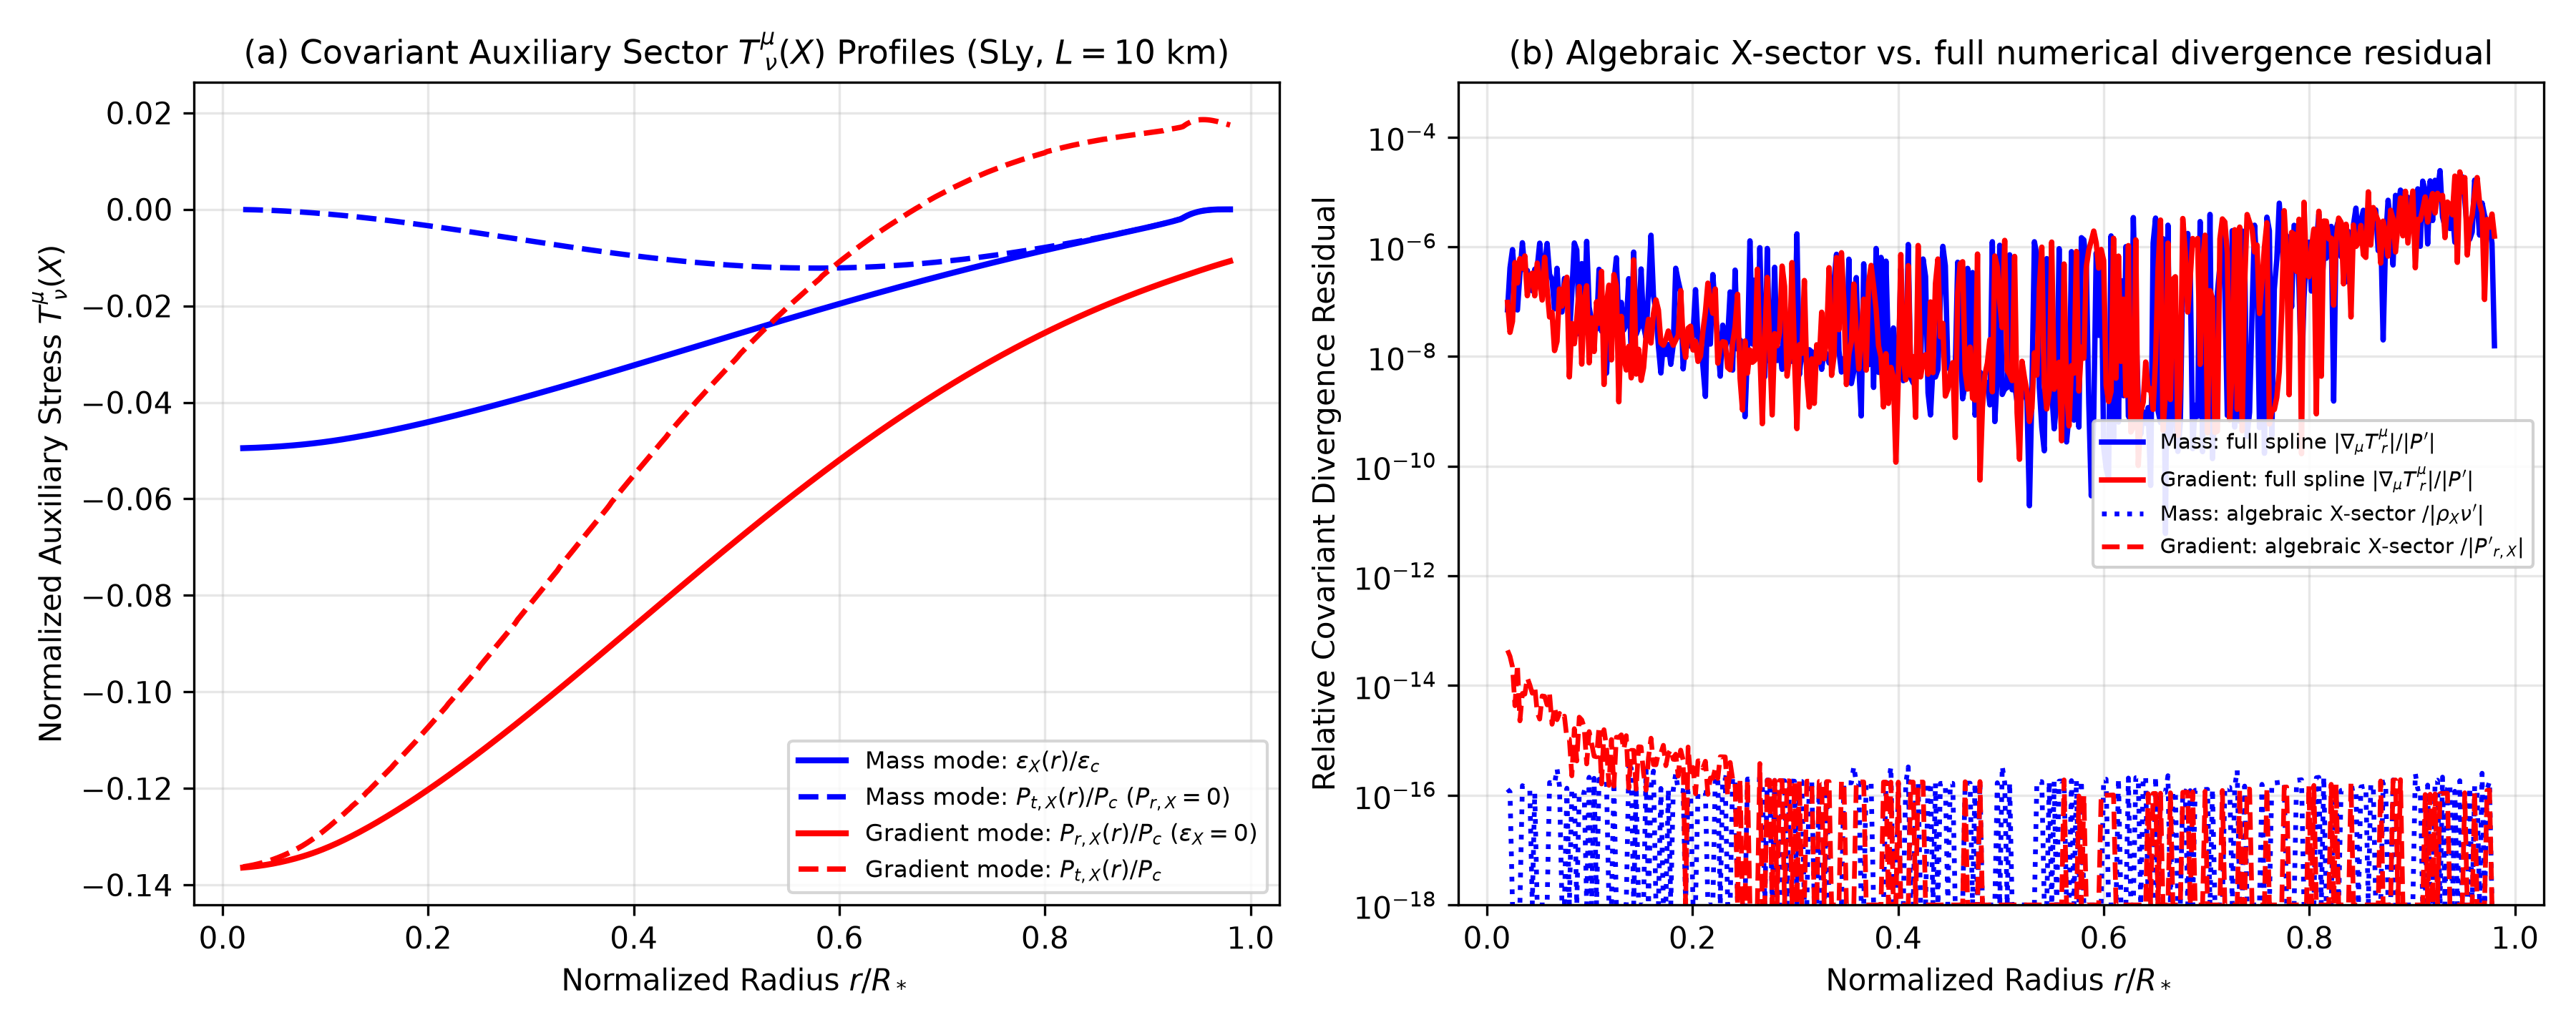
\includegraphics[width=0.70\linewidth]{fig3_conservation_check.png}\vspace{-3mm}
\caption{(a) Auxiliary stress-energy components $T^\mu_{\;\nu}(X)$ and (b) relative covariant divergence residuals $|\nabla_\mu T^\mu_{\;r}|/|P'|$ for SLy at $L=10\,\text{km}$, $\log_{10}\rho_{0c}=15.0$.}
\end{figure}

\begin{figure}[ht!]
\centering
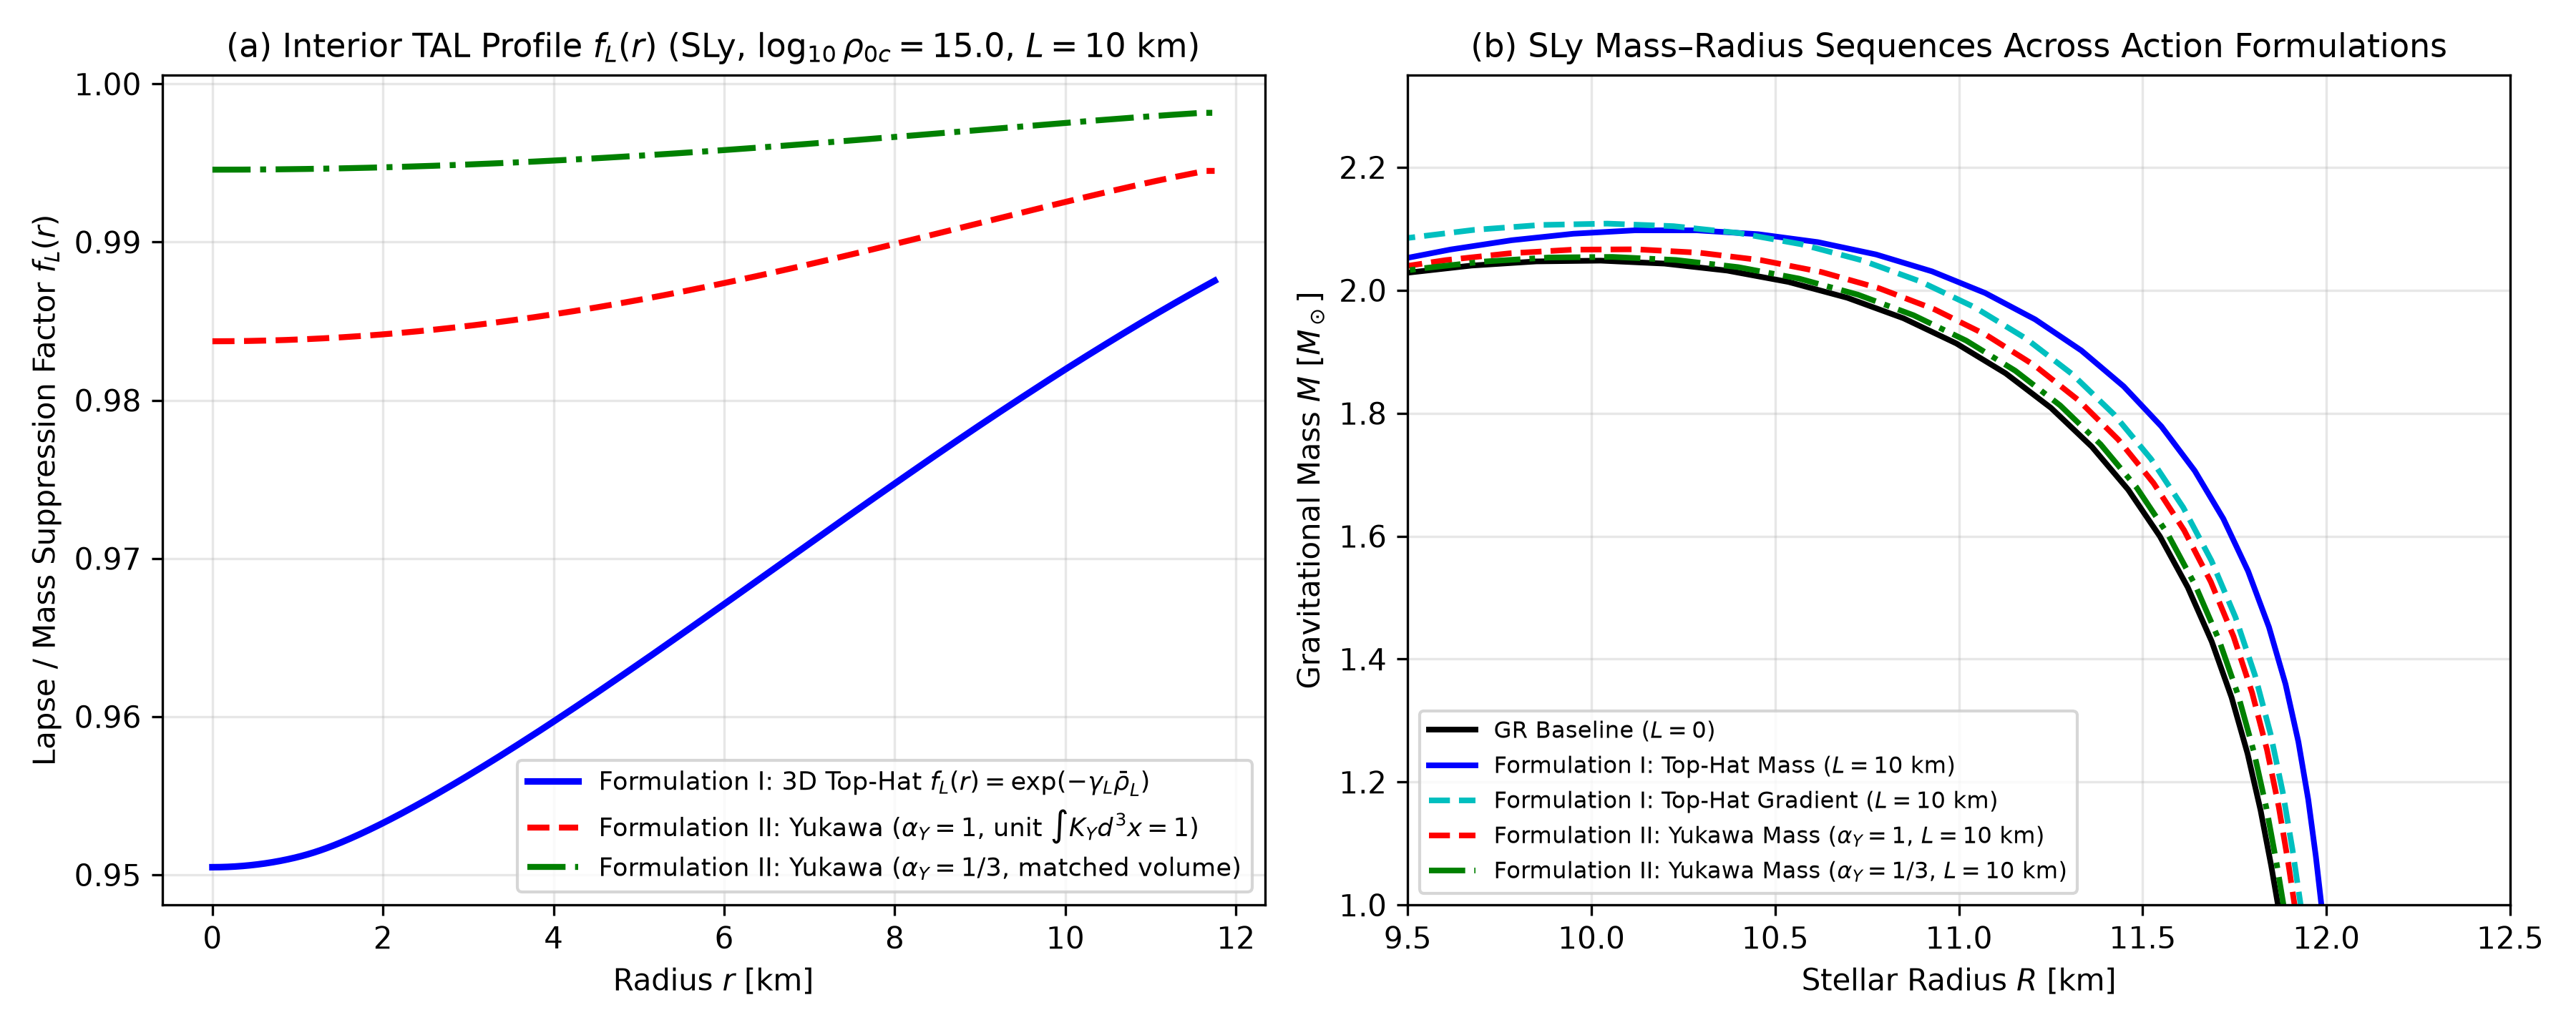
\includegraphics[width=0.70\linewidth]{fig1_action_profiles.png}\vspace{-3mm}
\caption{(a) Interior suppression factor $f_L(r)$ at $\log_{10}\rho_{0c}=15.0$ and (b) SLy mass--radius curves at $L=10\,\text{km}$ comparing Formulation I (3D top-hat) and Formulation II (screened Yukawa, $\alpha_Y=1$ and $\alpha_Y=1/3$).}
\end{figure}

\section{Static Nonlocal Tangent Model and Quasi-Dynamic BVP Test on the V21 Background}
In the V21 study (DOI \texttt{10.5281/zenodo.23602501}), radial stability was explored using two approximate \emph{frozen-$f_L$} ($\delta f_L = 0$) Sturm--Liouville operators (\texttt{matter} and \texttt{metric}). To understand why both frozen-$f_L$ operators miss the static mass peak $dM/d\rho_c = 0$, I first computed in \texttt{SymPy} the exact difference between the frozen-$f_L$ Chandrasekhar Sturm--Liouville operator $\mathcal{L}_{\text{SL}}^{\text{matter}}[\xi]$ and the linearized hydrostatic operator $\mathcal{H}_{\text{lin}}[\xi] = (\delta P)' + (\delta\varepsilon+\delta P)\nu' + (\varepsilon+P)\delta\nu'\big|_{\delta f_L=0}$ in mass mode:
\begin{equation}
  \mathcal{L}_{\text{SL}}^{\text{matter}}[\xi] - \sqrt{\frac{r}{r-2m}}\,e^{2\nu}\,\mathcal{H}_{\text{lin}}[\xi]\Big|_{\delta f_L=0} = \frac{4\pi r^{5/2}(f_L - 1)\Gamma P \varepsilon e^{2\nu}}{(r - 2m)^{5/2}}\Big[(4\pi r^3 P - 3r + 7m)\xi - r(r-2m)\xi'\Big]. \label{eq:factored_diff}
\end{equation}
Equation~\eqref{eq:factored_diff} vanishes identically when $f_L = 1$ (GR), because Chandrasekhar's integration by parts substitutes the GR Einstein identity $\lambda' + 2\nu' = 8\pi r e^\lambda(\varepsilon+P)$. When $f_L \ne 1$, however, $\lambda' + 2\nu' = 8\pi r e^\lambda(f_L\varepsilon + P)$, producing the $(f_L-1)$ residual in Eq.~\eqref{eq:factored_diff} AND omitting the nonlocal perturbation $\delta f_L[\delta\varepsilon,\xi]$.

I linearize (around the V21 \texttt{dense\_profile} background, not the new branches) the coupled system in terms of the enthalpy perturbation $\delta h(r) = \delta P/(\varepsilon+P)$ and mass perturbation $\delta m(r)$ on a radial grid locked to the exact piecewise-polytrope transition radii $r_{\text{trans}}$, including the nonlocal kernel perturbation operator:
\begin{equation}
  \delta f_L(r_i) = -\gamma_L f_L(r_i)\sum_j K_{ij}\,\frac{\varepsilon(r_j)+P(r_j)}{c_s^2(r_j)}\,\delta h(r_j), \qquad
  \begin{cases}
    \dfrac{d(\delta h)}{dr} = -\delta\nu'\!\left[\delta h, \delta m, \delta f_L[\delta h]\right] + \omega_0^2\,e^{\lambda-2\nu}\xi, \\[4pt]
    \dfrac{d(\delta m)}{dr} = 4\pi r^2\!\left[f_{\text{mass}}\frac{\varepsilon+P}{c_s^2}\delta h + \varepsilon\,\delta f_{\text{mass}}[\delta h]\right].
  \end{cases} \label{eq:coupled_bvp}
\end{equation}
At $\omega_0^2 = 0$, Eq.~\eqref{eq:coupled_bvp} is the exact tangent operator to the static equilibrium equations with respect to $\log_{10}\rho_{0c}$. As shown in Table 2 and Figure 3, the coupled problem~\eqref{eq:coupled_bvp} along the SLy $L=10\,\text{km}$ sequences has its zero at $\sim 7\times 10^{-5}\,\text{dex}$ from $dM/d\rho_c=0$ (equal to the pure-GR discretization baseline $7.12\times 10^{-5}\,\text{dex}$). Because at $\omega_0^2=0$ the problem reduces to $\mathcal{H}_{\text{lin}}[\delta h]=0$, this agreement verifies the \emph{static} nonlocal linearization, not the dynamical inertia: rescaling $W\to 4W$ at $\log_{10}\rho_{0c}=15.30427$ gives $\omega^2_{4W}/\omega^2_W = 0.2500$ ($\omega^2_W=4.897\times 10^{6}\,\text{s}^{-2}$) with identical shooting function $F(0)=0.023252$, so the zero crossing is inertia-invariant. The raw BVP inertia matrix $W$ is not symmetric; the symmetrized Galerkin form $\mathbf{M}_{\text{sym}} = \mathbf{D}^{T}\mathrm{diag}(w\,\Delta r)\mathbf{D}$ is symmetric with $\min\mathrm{diag}\,\mathbf{M}_{\text{sym}} = 5.68\times 10^{-9}>0$, a Gram-matrix property, not proof of a positive-definite physical kinetic Hessian. The column \texttt{omega0\_sq\_sym\_tangent\_s2} gives the first-order tangent estimate $\omega^2\simeq -F(0)/F'(0)$.

\begin{table}[ht!]
\centering
\caption{Radial stability zero-crossing densities ($\omega_0^2 = 0$) vs.\ the static turning point $dM/d\rho_c = 0$ along the SLy sequences ($L=0$ GR and $L=10\,\text{km}$ in \texttt{mass} and \texttt{gradient} modes) from \texttt{coupled\_stability\_results.csv} and \texttt{conservation\_Residuals.json}.}
\vspace{2pt}
\resizebox{\linewidth}{!}{%
\begin{tabular}{@{}lcccccc@{}}
\toprule
Sequence & Static Turning Point & Frozen-$f_L$ \texttt{matter} & Frozen-$f_L$ \texttt{metric} & Frozen-$f_L$ BVP & \textbf{Static tangent model (V21 bg)} & Mismatch Reduction \\
(SLy EOS) & $\log_{10}\rho_{0c}$ ($dM/d\rho_c=0$) & $\Delta\log_{10}\rho_{0c}$ [dex] & $\Delta\log_{10}\rho_{0c}$ [dex] & $\Delta\log_{10}\rho_{0c}$ [dex] & $\mathbf{\Delta\log_{10}\rho_{0c}}$ \textbf{[dex]} & Factor (vs.\ \texttt{matter} / BVP) \\
\midrule
GR ($L=0\,\text{km}$)           & $15.302445$ & $+2.91\times 10^{-7}$ & $+2.91\times 10^{-7}$ & $+7.12\times 10^{-5}$ & $\mathbf{+7.12\times 10^{-5}}$ & Baseline ($f_L \equiv 1$) \\
Mass ($L=10\,\text{km}$)        & $15.308269$ & $-1.34\times 10^{-3}$ & $+1.64\times 10^{-2}$ & $-4.06\times 10^{-3}$ & $\mathbf{+6.97\times 10^{-5}}$ & $\mathbf{19.2\times} \;/\; \mathbf{58.3\times}$ ($235.3\times$ vs.\ \texttt{metric}) \\
Gradient ($L=10\,\text{km}$)    & $15.298753$ & $-3.57\times 10^{-3}$ & $-3.17\times 10^{-4}\;^*$ & $-4.39\times 10^{-3}$ & $\mathbf{+7.39\times 10^{-5}}$ & $\mathbf{48.3\times} \;/\; \mathbf{59.3\times}$ (positive weight) \\
\bottomrule
\end{tabular}}\par\vspace{1pt}
{\scriptsize $^*$In gradient mode at $L=10\,\text{km}$, the approximate frozen-$f_L$ \texttt{metric} operator develops an indefinite weight $\mathcal{W}(r)\le 0$ near the surface; the static tangent model~\eqref{eq:coupled_bvp} uses a positive Gram weight (not a proof of kinetic positivity).}
\end{table}

\begin{figure}[ht!]
\centering
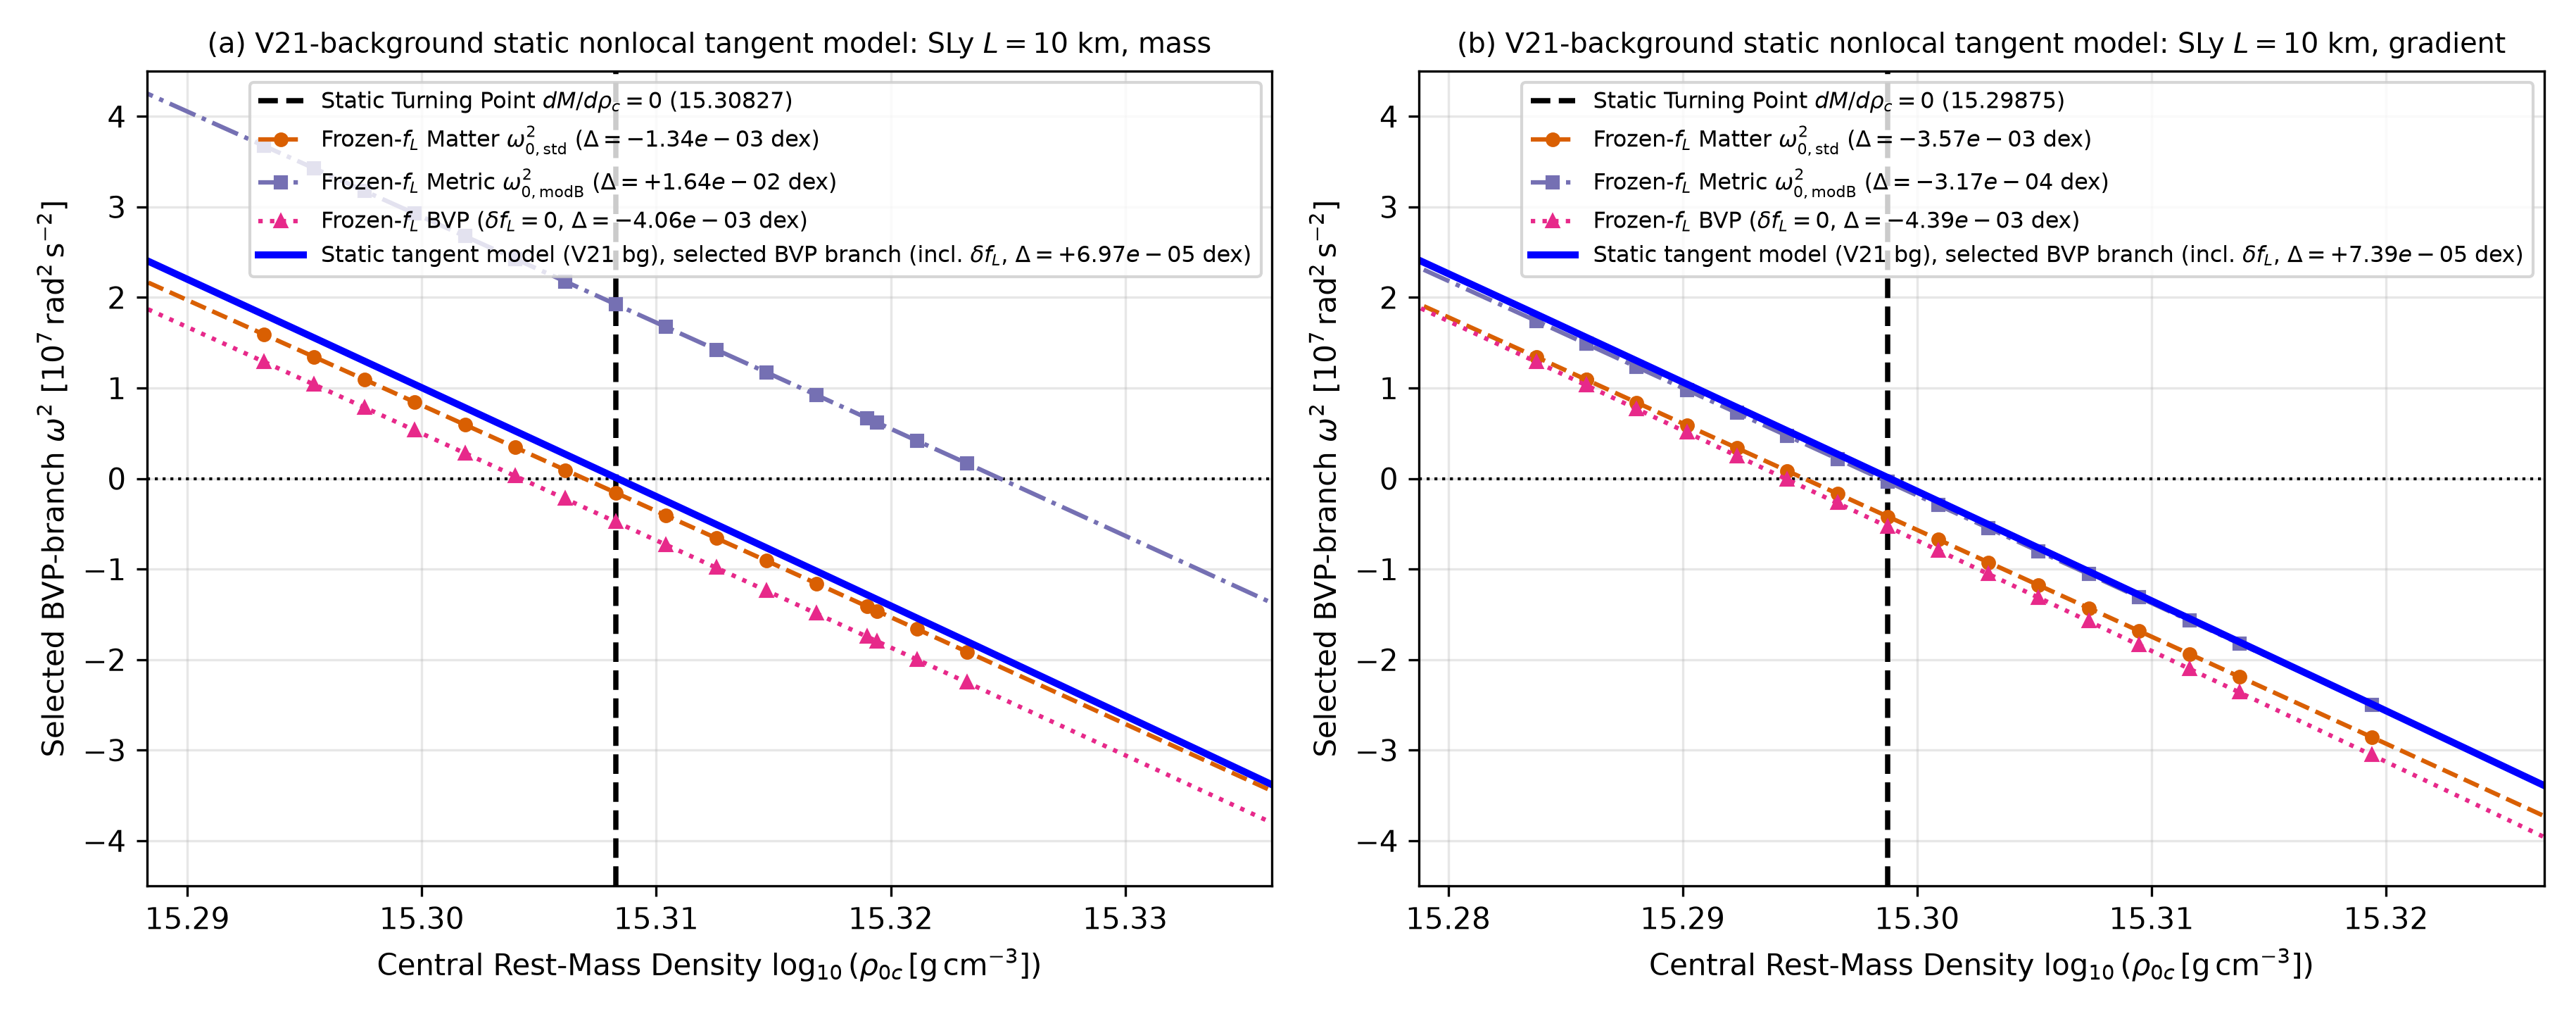
\includegraphics[width=0.70\linewidth]{fig2_coupled_stability.png}\vspace{-3mm}
\caption{V21-background static nonlocal tangent model: selected BVP-branch eigenvalue $\omega^2(\rho_{0c})$ across the static turning point $dM/d\rho_c = 0$ for SLy at $L=10\,\text{km}$ in (a) \texttt{mass} mode and (b) \texttt{gradient} mode, comparing the three uncoupled frozen-$f_L$ operators against the static tangent model (V21 bg).}
\end{figure}

\section{Microscopic Clock and Photon Coupling from the Action (H0 vs.\ H1)}
The covariant action framework makes transparent what determines the choice between observational hypotheses \textbf{H0} and \textbf{H1} for atomic clocks and stellar spectral lines. Let $\Psi_{\text{atomic}} = (\psi_e, A_\mu)$ denote the Dirac electron and Maxwell electromagnetic fields of an atomic clock at rest with the baryonic fluid four-velocity $u^\mu$, coupled to the effective Jordan-frame metric $\tilde{g}_{\mu\nu}[\phi_L]$:
\begin{itemize}\setlength{\itemsep}{1pt}\setlength{\parskip}{0pt}
  \item \textbf{Minimal / Purely Auxiliary Coupling ($\tilde{g}_{\mu\nu} = g_{\mu\nu}$ for $\Psi_{\text{atomic}}$ $\implies$ Hypothesis H0):} If $\phi_L$ couples only to the bulk baryonic fluid stress-energy tensor while atomic electrons and photons propagate on the physical spacetime metric $g_{\mu\nu}$, the proper time ticked by an atomic clock at $r = R_*$ is $d\tau_{\text{clock}} = \sqrt{-g_{00}(R_*)}\,dt = e^{\Phi_{\text{eff}}(R_*)/c^2}dt$. The surface redshift is purely metric ($1+z_{\text{H0}} = e^{-\Phi_{\text{eff}}(R_*)/c^2}$), with no direct $f_L(R_*)$ multiplier.
  \item \textbf{Universal Disformal Lapse or Conformal Jordan Coupling ($\tilde{g}_{\mu\nu} = g_{\mu\nu} + \frac{1 - f_L^2(\phi_L)}{c^2}u_\mu u_\nu$ $\implies$ Hypothesis H1):} If atomic clocks experience the disformal metric $\tilde{g}_{\mu\nu}$ whose comoving time-time component is $\tilde{g}_{00} = -1 + (1-f_L^2) = -f_L^2$ for $g_{00}=-1$, $u_0=-c$ (\texttt{SymPy} check \texttt{sym\_disformal\_g00\_residual} $=0$), the proper time increment of an atomic transition is $d\tilde{\tau}_{\text{clock}} = f_L(R_*)\,e^{\Phi_{\text{eff}}(R_*)/c^2}dt$. Photons propagating to infinity on null geodesics conserve coordinate frequency, yielding the direct surface clock factor $1+z_{\text{H1}} = e^{-\Phi_{\text{eff}}(R_*)/c^2}\,f_L(R_*)^{-1}$.
\end{itemize}
Table 3 summarizes the resulting numerical predictions from \texttt{clock\_coupling\_H0\_H1.csv} for Sirius B ($M=1.018\,M_\odot$, $R_*=5586.5\,\text{km}$, $n=3$ polytrope) and for the V20 $8558\,\text{kg}$ movable granite chamber ($\rho=2750\,\text{kg/m}^3$, $V_{\text{tot}}=3.1120\,\text{m}^3$). Because Sirius B leaves sub-megameter scales $L \lesssim 10^6\,\text{m}$ unconstrained even under H1, both H0 and H1 remain viable at neutron-star ($L \sim 1\text{--}10\,\text{km}$) and terrestrial laboratory ($L \sim 1\,\text{m}$) scales, with the V20 granite chamber directly testing the H1 clock branch at $|\Delta y_{\text{H1}}| = 1.436\times 10^{-24}$ ($L=1.0\,\text{m}$).

\begin{table}[ht!]
\centering
\caption{Quantitative comparison of action-derived clock couplings \textbf{H0} ($\tilde{g}_{\mu\nu}=g_{\mu\nu}$) and \textbf{H1} (disformal lapse $\tilde{g}_{00}=f_L^2 g_{00}$) for Sirius B ($n=3$) and the V20 $8558\,\text{kg}$ granite chamber from \texttt{clock\_coupling\_H0\_H1.csv}.}
\vspace{2pt}
\resizebox{\linewidth}{!}{%
\begin{tabular}{@{}lrrrrrrr@{}}
\toprule
System & $L$ [m] & $f_L(R_*)$ Top-Hat & $f_L(R_*)$ Yukawa & H0 Prediction & H1 Top-Hat Pred. & H1 Yukawa Pred. & Unit \\
\midrule
Sirius B ($1.018\,M_\odot$) & $1.0\times 10^3$ & $1.000000$ & $1.000000$ & $80.70055$ & $80.70055$ & $80.70055$ & km/s \\
Sirius B ($1.018\,M_\odot$) & $1.0\times 10^4$ & $1.000000$ & $1.000000$ & $80.70055$ & $80.70055$ & $80.70055$ & km/s \\
Sirius B ($1.018\,M_\odot$) & $1.0\times 10^6$ & $1.000000$ & $1.000000$ & $80.69839$ & $80.70094$ & $80.74476$ & km/s \\
Sirius B ($1.018\,M_\odot$) & $5.0\times 10^6$ & $0.999984$ & $0.999993$ & $80.69487$ & $85.38911$ & $82.85137$ & km/s \\
\midrule
V20 Granite ($8558\,\text{kg}$) & $0.50$ & $1.000000$ & $1.000000$ & $+3.075\times 10^{-48}$ & $-3.318\times 10^{-25}\;(-3.318\times 10^{-25})$ & $-2.008\times 10^{-25}\;(-1.943\times 10^{-25})$ & $\Delta y$ \\
V20 Granite ($8558\,\text{kg}$) & $0.85$ & $1.000000$ & $1.000000$ & $+1.208\times 10^{-47}$ & $-1.303\times 10^{-24}\;(-1.303\times 10^{-24})$ & $-3.373\times 10^{-25}\;(-3.101\times 10^{-25})$ & $\Delta y$ \\
V20 Granite ($8558\,\text{kg}$) & $1.00$ & $1.000000$ & $1.000000$ & $+1.331\times 10^{-47}$ & $-1.436\times 10^{-24}\;(-1.436\times 10^{-24})$ & $-3.781\times 10^{-25}\;(-3.407\times 10^{-25})$ & $\Delta y$ \\
\bottomrule
\end{tabular}}\par\vspace{1pt}
{\scriptsize V20 rows: H0 column = TAL excess over Newtonian GR at IN ($\mathbf{r}=\mathbf{0}$); H1 columns = IN shift (IN$-$OUT differential, $D_{\text{out}}=2.0\,\text{m}$). Newtonian GR: $\Phi_N(\text{IN})/c^2 = -9.269\times 10^{-24}$, IN$-$OUT $= -6.094\times 10^{-24}$; $\sigma_y=10^{-18}$ is an illustrative benchmark. Sirius B on the common effective-mass proxy (fixed $n=3$ Lane--Emden profile with the H0 effective-mass shift, not a newly solved equilibrium) gives at $L=10^3\,\text{km}$ H0 $80.69839$, H1 top-hat $80.69878\,\text{km/s}$.}
\end{table}

\noindent{\scriptsize\color{slate}\textbf{Archival References:} D.\ Szabolcsi, Zenodo DOIs \texttt{10.5281/zenodo.23217189} (V14), \texttt{10.5281/zenodo.19666220} (V17), \texttt{10.5281/zenodo.23497128} (V19), \texttt{10.5281/zenodo.23540741} (V20), \texttt{10.5281/zenodo.23602501} (V21), and \texttt{10.5281/zenodo.23604423} (V22 Book Edition).}

\end{document}
